\documentclass[pdf]{beamer} 

\usepackage[utf8]{inputenc} 
\usepackage{graphicx} 
\usepackage[squaren, Gray]{SIunits} 
\usepackage{amsmath}  

\usetheme{warsaw} 
\mode<presentation>{} 
 
\title{Physique} 
\subtitle{APP 3 : Rayonnement électromagnétique} 
\author{Groupe 1243} 
 
\begin{document} 

\begin{frame} 
	\titlepage 
\end{frame} 
  
% --------------------
% Question 1
% -------------------
\begin{frame}{Courant alternatif dans une antenne}
	On peut comparer notre antenne à un condensateur.

	\begin{figure}[htb!] 
		\centering
		\begin{subfigure}
			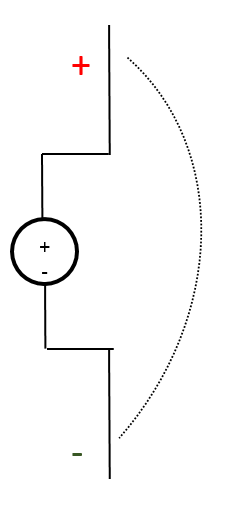
\includegraphics[scale=0.5]{circuit-antenne.png}
		\end{subfigure}
		\begin{subfigure}
			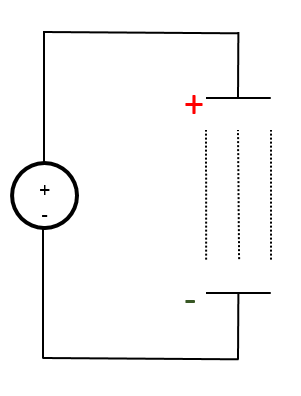
\includegraphics[scale=0.5]{circuit-antenne-2.png}
		\end{subfigure}
		\caption{Circuit d'une antenne.}
	\end{figure}
\end{frame}

% --------------------
% Question 1
% -------------------
\begin{frame}{Largeur des antennes}
	\begin{figure}[ht!] 
		\centering  
		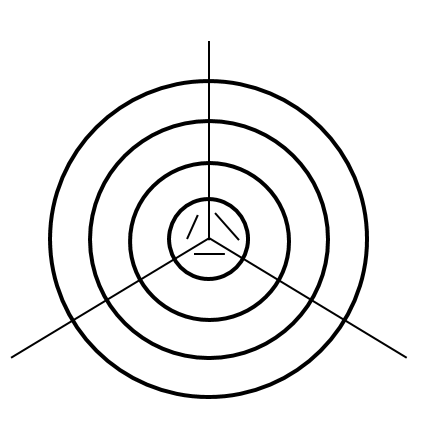
\includegraphics[scale=0.30]{antennes.png}  
		\caption{Coupe horizontale d'une antenne.}  
	\end{figure}  
 	
	Diffraction d'une fente rectangulaire :
	$$I_d (P) \propto I_0 \left[\frac{\sin\pi\frac{a\sin\theta}{\lambda}}{\pi\frac{a\sin\theta}{\lambda}}\right]^2$$
	On impose une intensité 2 fois plus faible aux limites du domaine des antennes.

	On obtient une largeur $a = \unit{0.171}{\meter}$.
\end{frame}

% --------------------
% Question 3
% -------------------
\begin{frame}{Antenne le long des autoroutes}
	On place deux antennes dans la même direction mais émettant leurs ondes dans des sens opposés.
\end{frame}

% --------------------
% Question 4
% -------------------
\begin{frame}{Directivité angulaire dans le plan vertical}
	Diffraction de N fentes rectangulaire s:
	$$I_d (P)\propto A^2 \left[\frac{\sin \pi \frac{a \sin \theta}{\lambda}}{\pi \frac{a \sin \theta}{\lambda}}\right]^2  
	\cdot \left[  \frac{\sin \pi \frac{N d \sin \theta}{\lambda}}{\pi \frac{d \sin \theta}{\lambda}}\right]^2$$

	Pour un une maison située à une distance $h$ d'un pylône de hauteur $h$ la largeur de la fente est proportionnelle à $3.3 \cdot 10^{-3}A^2$.
\end{frame}

% --------------------
% Question 5
% -------------------
\begin{frame}{Comparaison entre l'antenne et sa longeur d'onde}
	A faire
\end{frame}

% --------------------
% Question 6
% -------------------
\begin{frame}{Puissance d'émission}
	Connaisant la formule de l'intensite:

	$$\frac{P}{S}=I=\epsilon_0 \cdot c \cdot E^2 $$\\ 

	$$P=\epsilon_0 \cdot c \cdot E^2 \cdot 4 \pi  r^2$$
	
	\begin{center}
		A \unit{50}{\meter} de l'antenne : $P= \unit{3.34}{\watt}$.
	\end{center}
\end{frame}

% --------------------
% Question 7
% -------------------
\begin{frame}{Champs électrique rayonné}
	Connaisant la formule de l'intensite :
	$$\frac{P}{S}=I=\epsilon_0 \cdot c \cdot E^2 $$\\

	$$E =\sqrt{\frac{P}{\epsilon_0 \cdot c \cdot 4\pi r^2}}$$

	A \unit{1}{\meter} de l'antenne : $P= \unit{10}{\volt\per\meter}$. 

	Pour notre fréquence, la norme autorisé est de \unit{20.6}{\volt\per\meter}.
\end{frame}

% --------------------
% Question 8
% -------------------
\begin{frame}{Polarisation des ondes émises par l'antenne}
	La polarisation est linéaire.
	% Des sources? Plus d'explications?
\end{frame}

% --------------------
% Question 1
% -------------------
\begin{frame}
	% TODO by NGillain
\end{frame}
\end{document}